\chapter{Progettazione e codifica del progetto}\label{cap:progettazione-codifica}

\intro{In questa sezione, saranno elencate le tecnologie principali utilizzate durante lo sviluppo del sistema oggetto del tirocinio.
Inoltre, verrà descritto il ciclo di vita del software, le fasi di progettazione e codifica e le scelte architetturali realizzate, 
a livello di sistema e design pattern.}

\section{Componenti principali del sistema}\label{sec:componenti-principali}
Il sistema risulta essere composto da due parti principali: 
\begin{itemize}
    \item{\textbf{Front-end}}: è la parte visibile all'utente, che permette di interagire con il sistema. È stata sviluppata utilizzando il framework React e il linguaggio TypeScript. 
    Questa comprende la parte grafica da me realizzata e la relativa interazione con il contratto fornito come libreria dallo studente Alessio De Biasi.
    \item {\textbf{Back-end}}: è la parte che gestisce la logica dell'applicazione, che permette di interagire con la blockchain e di gestire le funzionalità del sistema. È stata sviluppata utilizzando il linguaggio Solidity.
    Quest'ultima comprende il contratto sviluppato dallo studente magistrale Alessio De Biasi basato sugli standard \glsfirstoccur{\gls{w3cg}} \glsfirstoccur{\gls{ssig}} e \glsfirstoccur{\gls{didg}}.
\end{itemize}

\section{Tecnologie utilizzate}\label{sec:tecnologie-strumenti}

\subsection{Codifica front-end}

\subsubsection{React}
React è una libreria JavaScript utilizzata per la creazione di interfacce utente. È stata sviluppata da Facebook e rilasciata nel 2013. 
Essa consente di creare dei componenti riutilizzabili che rappresentano parti dell'interfaccia e gestire lo stato dell'applicazione in modo efficiente e scalabile.
Questo lo rende adatto allo sviluppo di applicazioni complesse e dinamiche (specifiche e riferimenti a \cite{site:react}).
Nel mio caso, è utilizzato per la progettazione delle componenti e delle pagine.

\subsubsection{TypeScript}
TypeScript è un linguaggio di programmazione open source sviluppato da Microsoft. È un super-set di JavaScript che aggiunge tipi statici opzionali al linguaggio,
permettendo di scrivere codice più robusto e manutenibile, grazie alla possibilità di definire interfacce e classi (secondo \cite{site:react}).
All'interno delle pagine realizzate, sono stati creati dei tipi appositi per poter gestire più facilmente le informazioni e le funzionalità del sistema.

\subsection{Codifica back-end}

\subsubsection{Solidity}
Solidity è un linguaggio di programmazione orientato agli oggetti per la scrittura di smart contract. È stato sviluppato da Ethereum e permette di gestire
lo stato di un contratto, definire funzioni e interagire con altri contratti all'interno delle blockchain,
grazie alla gestione del sistema di transazioni basato sugli eventi e alla possibilità di definire interfacce (in base a quanto presente in \cite{site:solidity}).
L'interazione con la blockchain e il contratto da richiamare come libreria è stato scritto in questo linguaggio.

\subsection{Librerie di terze parti}

\subsubsection{Node.js}
Node.js è un ambiente di runtime open source per l'esecuzione di codice JavaScript lato server. È basato sul motore JavaScript V8 di Google Chrome e permette di gestire
le dipendenze dell'applicazione, grazie al suo package manager \textit{npm}, differenziando le librerie dell'applicazione e quelle di terze parti.
Tramite semplici comandi, è possibile installare e rimuovere le dipendenze, aggiornarle e gestire le versioni. 
Lo strumento ha permesso una facile configurazione delle dipendenze e la gestione delle versioni (riferimenti in \cite{site:node}).

\subsubsection{web3.js}
web3.js è una collezione di librerie JavaScript per poter interagire facilmente con le blockchain, in particolare con Ethereum.
Essa permette di connettersi ad un nodo della blockchain, inviare transazioni e interagire con gli smart contract, gestendo facilmente il collegamento
e l'interazione tra la parte grafica e gli smart contract, definendo modularmente le funzionalità presenti (secondo riferimenti in \cite{site:web3}).
Grazie a questo, è stato possibile gestire facilmente l'interazione con la blockchain e gli smart contract, permettendo la chiamata al contratto
e alle sue funzioni.

\subsubsection{Hardhat}
Hardhat è un ambiente di sviluppo per le blockchain che permette di testare e distribuire smart contract. Esso permette di distribuire facilmente
in locale una blockchain, per poter testare le funzionalità degli smart contract, e di distribuire gli smart contract su una blockchain pubblica, come ad esempio
Ethereum (in base alle definizioni e guide in \cite{site:hardhat}).

\subsection{Versionamento}

\subsubsection{GitHub}
GitHub è una piattaforma di hosting per progetti software. Essa permette di gestire il versionamento del codice tramite il sistema di controllo di versione Git.
In particolare, consente lo sviluppo di codice mantenendo un \textit{repository} remoto, che permette di gestire le modifiche e le versioni del codice, mantenendo un registro
delle modifiche effettuate e permettendo di tornare ad una versione precedente del codice (riferimenti di massima in \cite{site:github}). 

\subsection{Verifica}

\subsubsection{ESLint}
ESLint è uno strumento di analisi statica del codice per identificare i modelli problematici trovati nel codice JavaScript.
È stato utilizzato per garantire la qualità del codice prodotto, tramite la definizione di regole e la segnalazione di eventuali errori.

\subsubsection{Jest}
Jest è un framework di test per JavaScript. È stato utilizzato per la definizione di test unitari e di integrazione, per verificare il corretto funzionamento
delle funzionalità implementate. 

\section{Configurazione ambiente di sviluppo}\label{sec:configurazione-ambiente}

\subsection{Smart Contract}
All'interno del mio progetto di stage, per realizzare l'implementazione degli smart contract, ho utilizzato un ambiente di sviluppo locale,
basato su \textit{Hardhat}, un ambiente di sviluppo per Ethereum che permette di testare e distribuire smart contract.
Tramite questo, è stato possibile permettere la creazione di un ambiente di test locale, tramite l'ausilio di alcuni \textit{script}, in
grado di gestire la compilazione e la successiva esecuzione (\textit{deploy}) del contratto fornito sulla rete locale.
Per poter effettuare le singole chiamate, lo strumento fornisce un insieme di account di test con un saldo iniziale di 10000 ETH (valute della rete Ethereum, riferimento dello strumento), 
che possono essere utilizzati per effettuare le chiamate desiderate qualora siano presenti transazioni (normalmente in esecuzione sulla porta 8545 all'interno della rete locale). \\

Nello specifico, la strutturazione prevede:
\begin{itemize}
    \item uno script di \textit{deploy}, scritto in TypeScript, che definisce il contratto che viene chiamato, il suo indirizzo sulla rete locale
    e la generazione di un file \textit{json} chiamato \textit{ABI}, che contiene le informazioni in formato binario del contratto. Esso viene utilizzato nella parte frontend;
    \item uno script di test, scritto in TypeScript, che permette di testare le funzionalità del contratto, tramite l'ausilio di \textit{web3.js};
    \item uno script di configurazione, che definisce l'account utilizzato sulla rete locale e le librerie presenti.
\end{itemize}

\subsection{Frontend}
Per lo sviluppo del front-end, ho utilizzato un ambiente di sviluppo locale, basato su \textit{Node.js}, un ambiente di runtime per JavaScript.
Tramite questo, è stato possibile gestire le dipendenze del progetto, tramite il package manager \textit{npm}, e avviare un server locale per poter testare
e scrivere le pagine presenti. In particolare, il server è stato avviato sulla porta 3000, per poter permettere l'interazione con il contratto tramite
le funzionalità del front-end e le chiamate al contratto.
Nello specifico, la strutturazione prevede:
\begin{itemize}
    \item una cartella \textit{src}, contenente i file \textit{.js} e \textit{.ts} che definiscono le funzionalità del front-end;
    \item una cartella \textit{public}, contenente i file \textit{.html} e \textit{.css} che definiscono le pagine del front-end;
    \item una cartella \textit{build}, contenente i file \textit{.js} e \textit{.ts} compilati, che vengono utilizzati per l'esecuzione del front-end;
    \item una cartella \textit{node\_modules}, contenente le dipendenze del progetto.
\end{itemize}

\newpage
\section{Progettazione}\label{sec:progettazione-requisiti}

\subsection{Architettura front-end}

L'utilizzo di React ha permesso di definire una struttura modulare per il front-end, in modo da poter definire facilmente le pagine e le funzionalità.
Esso è formato da un insieme di componenti, che definiscono un insieme di funzioni riutilizzabili, ognuna delle quali definisce un suo comportamento. 
La logica dell'applicazione permette di gestire singolarmente le funzionalità del codice, definendo le pagine come funzioni che vengono
esportate e utilizzate come entità indipendenti. In questo modo, si incrementa la modularità del codice e la sua manutenibilità, in quanto ogni componente
o pagina può essere riutilizzato in modo semplice e può essere modificato senza influenzare il resto del codice. \\

La struttura della pagina HTML è stata definita tramite \textit{TSX}, un'estensione di \textit{React} che permette di definire la struttura della pagina 
in collaborazione con \textit{HTML} e \textit{CSS} e il linguaggio di programmazione \textit{TypeScript}.
Tramite l'utilizzo dei cosiddetti \textit{hook}, è stato possibile definire le funzionalità del front-end, in modo da poter gestire le chiamate tra le componenti della 
pagina in base all'attivazione di specifici eventi in modo dinamico, grazie all'uso degli \textit{state}.
In questo modo, i singoli componenti e le pagine, definite come viste, riescono ad avere singola responsabilità e a poter essere riutilizzate in modo semplice. \\

La logica viene mantenuta separata dalla presentazione, utilizzando la strutturazione a componenti in grado di comunicare nativamente con il 
DOM (Document Object Model), permettendo di definire la struttura della pagina in modo dinamico e di poter gestire le interazioni con l'utente
solo tramite le componenti e le pagine stesse, separando la presentazione offerta tramite \textit{HTML} e \textit{CSS} dalla logica del front-end strutturata
a funzionalità. \\

Dato che React è una libreria grafica, non viene forzato alcun preciso pattern architetturale, ma viene lasciata libertà di scelta allo sviluppatore.
In questo caso, il pattern utilizzato è il \textit{Flux Pattern}, che permette di definire un flusso unidirezionale dei dati, in modo da poter gestire
le interazioni dell'utente con la pagina e le chiamate al contratto in modo semplice e senza dover gestire la sincronizzazione dei dati tra le varie componenti.
Ciò permette all'applicazione di essere gestita da funzionalità precise a cascata, andando ad interagire con l'esterno con semplici aggiunte di moduli o dipendenze.
Come visibile dalla figura \ref{fig:react}, la logica si compone di un componente radice che descrive l'applicazione,
a sua volta costituita eventualmente da uno o più componenti, innestati a vari livelli secondo la relazione di composizione,
includendo anche eventuali componenti di terze parti per permettere la gestione e l'interazione all'esterno, esportando la funzionalità utile.

\begin{figure}[h]
    \centering
    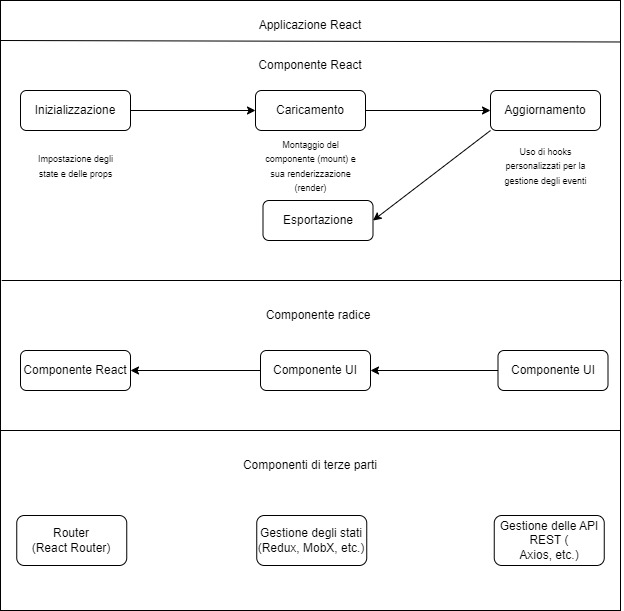
\includegraphics[width=0.6\textwidth, alt={Descrizione dello schema logico di un'applicazione React}]{immagini/react.jpeg}
    \caption{Schema logico applicazione React} \label{fig:react}
\end{figure}

\newpage

Secondo le \textit{best practices} di React, è stato utilizzato il pattern \textit{Functional Component}, che permette di definire proprietà specifiche (definite come \textit{props})
ed uno stato interno in grado interagire con eventi asincroni da parte dell'utente. La strutturazione si compone di un insieme di funzioni e stati definiti
al caricamento della pagina (utilizzando l'\textit{Hook Pattern}, attraverso gli \textit{hooks} \textit{useEffect} e \textit{useState}), in grado di caricare e gestire dinamicamente le informazioni
al suo interno, esportando poi il componente funzionale o la stessa pagina, secondo un insieme di funzionalità definite dallo specifico contesto. \\

Nello specifico, l'applicazione definisce per ogni pagina una cartella comprensiva del componente funzionale
esportato e del suo stile, e un file di test per verificare le principali funzionalità previste.
Inoltre, è presente una cartella \textit{components}, contenente i componenti utilizzati da tutte le pagine comrpensive dei dati del sito e dell'autenticazione, e
una cartella \textit{utils}, contenente le funzionalità definite all'avvio dell'applicazione.
L'autenticazione viene gestita tramite un contesto, definito dal design pattern \textit{Provider Pattern} di React, che permette di definire un contesto globale
in cui tutta l'applicazione può accedere, in modo da poter gestire le informazioni dell'utente e le sue credenziali in modo sicuro e globale. 
Le singole opzioni visibili tra utente autenticato e non, sono invece gestite secondo il pattern \textit{Conditional Rendering}, in grado di differenziare le opzioni
visibili in base al suo stato. 


\subsection{Architettura back-end}

\section{Codifica}\label{sec:codifica-requisiti}

\subsection{Codifica front-end}

\subsection{Codifica back-end}